\chapter{实验设计及结果分析}\label{chap:method}

本章节针对基于AllDiff-LS算法实现的求解工具设计了实验,并对实验结果进行了分析。章节主要包含三部分:第一部分介绍实验安排,比如采用的数据集、比较的方法等;第二部分介绍算法在多个实验基准上同其他方法的性能比较;第三部分对实验中提到的各种策略的有效性进行消融实验。

\section{实验设置}
\textbf{实验样例:}在本章节,本文选择了四个经典问题作为基准:数独,N皇后,全间隔和二正交拉丁方(2-MOLS)问题\cite{colbourn2001mutually}。它们都可以使用AllDifferent约束进行建模,并且这些问题的约束生成的ACG具有独特的特征,使这些问题极具代表性。下面,本文给出这些问题的编码的具体细节。

\begin{definition}[数独]
一个\textit{数独(Sudoku)}问题实例$\mathcal{S}^n$可以用一个$n^2 \times n^2$的网格表示,其中填充着1到$n^2$范围内的数字,这里$n$被称为问题的\textit{阶数}。
网格被划分为$n^2$个大小为$n \times n$的子网格。通常一些单元格已经被固定为特定的值。问题要求每单元格中的数字满足每行、每列和每个子网格中每个数字恰好出现一次。
\end{definition}

在数独问题中,所有变量表达式都是单变量表达式,并出现在多个AllDifferent约束中。以下为其编码:
\begin{align*}
    &\texttt {AllDifferent} (x_{i,1}, x_{i,2}, \dots, x_{i,n^2}) \text{  for } 1 \leq i \leq n^2, & \\
    &\texttt {AllDifferent} (x_{1,j}, x_{2,j}, \dots, x_{n^2,j}) \text{  for } 1 \leq j \leq n^2, & \\
    &\texttt {AllDifferent} (x_{i*n+u,j*n+v} \mid \text{ for } 1 \leq u,v \leq n) \text{  for } 0 \leq i, j \leq n-1, & \\
    &x_{i, j} \in\{1, 2, \dots, n^2\} \text { for } 1 \leq i, j \leq n^2.&
\end{align*}%

\begin{definition}[N皇后]
一个\textit{N皇后(N-queens)}问题实例$\mathcal{Q}^n$是将$n$个皇后放置在一个$n \times n$的棋盘上,使得没有皇后互相攻击(任何两个皇后都不能处于同一行、同一列或同一对角线上),这里$n$被称为问题的\textit{阶数}。
\end{definition}

在N皇后问题中,一个变量可以有多个变量表达式,但是每个变量表达式只存在于一个AllDifferent约束中。建模这个问题的一种方法是为每一行引入一个整数变量$x_i$,其中$i = 1, 2, \dots, n$,它的取值范围是从列1到$n$。这意味着在每一行$i$中,皇后被放置在第$x_i$列上。以下为其编码:
\begin{align*}
    &\texttt {AllDifferent} (x_{1}, x_{2}, \dots, x_{n}), & \\
    &\texttt {AllDifferent} (x_{1}-1, x_{2}-2, \dots, x_{n}-n), & \\
    &\texttt {AllDifferent} (x_{1}+1, x_{2}+2, \dots, x_{n}+n), & \\
    &x_{i} \in\{1, 2, \dots, n\} \text { for } 1 \leq i \leq n.&
\end{align*}%


\begin{definition}[全间隔]
一个\textit{全间隔(All-Interval)}问题实例,表示为 $\mathcal{A}^n$,涉及将 $n$ 个不同的元素排列成一个序列,使得任意两个元素之间的绝对差形成一个包含所有可能整数从 1 到 $n-1$ 的集合。$n$ 的值被称为问题的\textit{阶数}。
\end{definition}

在全间隔问题中,仅存在两个AllDifferent约束,变量和变量表达式之间是多对多的关系,并且一个变量可能在一个约束中的两个变量表达式中出现。问题建模的形式化表示如下:
\begin{align*}
    &\texttt {AllDifferent} (x_{1}, x_{2}, \dots, x_{n}), & \\
    &\texttt {AllDifferent} (|x_{1}-x_{2}|, |x_{2}-x_{3}|, \dots, |x_{n-1}-x_{n}|), & \\
    &x_{i} \in\{1, 2, \dots, n\} \text { for } 1 \leq i \leq n.&
\end{align*}%

\begin{definition}[互正交拉丁方]
\textit{互正交拉丁方(MOLS)}是由数学家欧拉提出的一个极具挑战性的组合问题。拉丁方阵可以看作没有子网格约束的数独问题。给定两个相同阶数$n$的拉丁方阵,如果它们在每个对应位置的元素组合是唯一的,那么它们是互相正交的,表示为$2$-$MOLS(n)$。
\end{definition}

在互正交拉丁方问题中,在采用AllDifferent约束进行建模的情况下,一个变量存在于多个变量表达式中,而且一个单一的变量表达式中包含多个变量,这些变量也出现在多个AllDifferent约束中。
因此,MOLS的AllDifferent约束图比前三种情况更为复杂。以下为其一种编码方式:
\begin{align*}
    &\texttt {AllDifferent} (x_{i,1}, x_{i,2}, \dots, x_{i,n}) \text{  for } 1 \leq i \leq n, & \\
    &\texttt {AllDifferent} (x_{1,j}, x_{2,j}, \dots, x_{n,j}) \text{  for } 1 \leq j \leq n, & \\
    &\texttt {AllDifferent} (y_{i,1}, y_{i,2}, \dots, y_{i,n}) \text{  for } 1 \leq i \leq n, & \\
    &\texttt {AllDifferent} (y_{1,j}, y_{2,j}, \dots, y_{n,j}) \text{  for } 1 \leq j \leq n, & \\
    &\texttt {AllDifferent} (x_{i,j}*n+y_{i,j} \mid \text{ for } 1 \leq i,j \leq n), & \\
    &x_{i, j}, y_{i, j} \in\{1, 2, \dots, n\} \text { for } 1 \leq i, j \leq n.&
\end{align*}%

虽然存在一些人工制作的实例\cite{mantere2008solving, zhang2021early},但这些实例的规模较小,相对容易解决。因此,本文主要生成大规模随机实例进行实验。
使用\cite{lewis2007metaheuristics}和\cite{musliu2017sudoku}中提到的方法,本文生成了从4到9阶的数独实例(即,从$16 \times 16$到$81 \times 81$的大小)。本文为每个固定单元格比例生成了100个实例,步长为10\%,从0\%到90\%,总共生成了6000个单独的实例,并使用`$\mathcal{S}$-$n$-$r$'来表示阶数为$n$、固定单元格比例为$r$的数独实例族。
对于N皇后问题,本文比较了从500到6000阶的十二个实例(步长为500),记为`$\mathcal{Q}$-$n$'。
对于全间隔问题,本文比较了从12到26阶的八个实例(步长为2),记为`$\mathcal{A}$-$n$'。
对于2-MOLS问题,由于其难度级别,本文只比较了阶数为3、4、5、7、8和9的六个实例(已经证明2-MOLS(6),也称为36官问题,没有解),记为`$\mathcal{L}$-$n$'。

\textbf{比较方法:}本文将AllDiff-LS与一个启发式求解器Yuck\footnote{https://github.com/informarte/yuck},以及两个完备求解器ILOG CPLEX Optimizer(版本20.10,简称CPLEX)和Choco(版本4.10.13)\cite{prud2019choco}进行了比较,所有这些都支持`AllDifferent'约束。Yuck采用了\cite{bjordal2015constraint}的想法,并在2022 MiniZinc挑战赛的局部搜索赛道中获得了冠军,而CPLEX和Choco分别是知名的商业和开源求解器,它们都支持各种化简策略。此外,对于数独,本文还比较了两个专用的启发式算法,来自\cite{lloyd2020antcolony}的蚁群算法(ACS)和来自\cite{musliu2017sudoku}的迭代局部搜索算法(ILS),其中ACS被调整为接受大于5的阶数。在ACS算法中,作者将约束传播和蚁群算法相结合,通过Minimum Remaining Values Heuristic搜索求解空间。而在ILS算法中,算法会在初始化时满足部分约束,并通过交换变量赋值的方式进行局部搜索。

\textbf{实验安排及指标:}后续所有实验都在一台配备有Intel Xeon Platinum 8153(2.00GHz)和2048G RAM的服务器上进行,系统为Centos 7.7.1908。每个算法在一个实例上的执行时间限制$T$为1000秒。启发式算法在每个实例上运行十次,其中支持随机种子(AllDiff-LS, ACS)的方法将使用不同的随机种子(从1到10)。其他算法在每个实例上只运行一次。对于每个算法,本文使用$R$来表示一个实例族的成功运行百分比,并使用$time$(以秒为单位)来表示其平均成功时间。当$R$为0时,其$time$被记录为`-'。

\textbf{实验结果展示:}根据上文提到的求解方法和求解样例,后续本文将比较这些求解器的求解性能,以及通过一系列消融实验来证明设计的算法框架中各个策略的有效性,具体指标为求解的成功率、比例和开销。


\section{AllDiff-LS求解AllDifferent约束的能力}

根据每个问题的特点,本文选择了具有代表性的基线方法进行比较,具体地,本文将问题实例分为了两类,第一类是数独,它是一类包含固定点的CSP,因此在搜索之前需要进行化简,而其他三类无固定点的CSP属于第二类。

关于数独,由于已经有专门的启发式算法性能优于一般的启发式求解器,本文没有展示Yuck的实验结果,其整体实验结果如\tablename~\ref{tab:sudoku}所示。可以观察到,在填充率超过70\%后,数独的难度急剧下降,所有算法都可以通过推理规则轻易找到解决方案。其中,ACS算法和ACP-LS算法的效率优于其他算法,这证明了ACP-LS减少规则的有效性。

当填充比例在40\%和60\%之间时,其求解难度最大。随着阶数的增加,本文选择的算法中没有一个算法能保证100\%的成功率。
尤其是当阶数高于5时,这些算法的求解性能开始恶化,出现无法解决的情况。而AllDiff-LS的性能下降较慢,直到最困难的9阶,它仍然可以在10秒内解决除填充比例在40\%-60\%范围外的每一个实例。

\begin{table*}[t]
    \bicaption{AllDiff-LS和其他最先进的基线方法在数独实例上的结果。}{Results of AllDiff-LS and other state-of-the-art baseline methods on Sudoku.}
    \label{tab:sudoku}
    \footnotesize
    \centering
    \setlength{\tabcolsep}{0.2mm}% column separation
    \renewcommand{\arraystretch}{1.2}%row space 
    \resizebox{\linewidth}{!}{
        \begin{tabular}{ccccccccccc|ccccccccccc}
            \hline
            Instance & \multicolumn{2}{c}{ACS} & \multicolumn{2}{c}{ILS} & \multicolumn{2}{c}{CPLEX} & \multicolumn{2}{c}{Choco} & \multicolumn{2}{c|}{AllDiff-LS} & 
            Instance & \multicolumn{2}{c}{ACS} & \multicolumn{2}{c}{ILS} & \multicolumn{2}{c}{CPLEX} & \multicolumn{2}{c}{Choco} & \multicolumn{2}{c}{AllDiff-LS} \\
            family  &  $R(\%)$ & $time$  &  $R(\%)$ & $time$  &  $R(\%)$ & $time$  &  $R(\%)$ & $time$  &  $R(\%)$ & $time$  &
            family  &  $R(\%)$ & $time$  &  $R(\%)$ & $time$  &  $R(\%)$ & $time$  &  $R(\%)$ & $time$  &  $R(\%)$ & $time$  \\
            \hline
            
            $\mathcal{S}$-4-0 & \textbf{100} & $0.04$ & \textbf{100} & $0.08$ & \textbf{100} & $18.50$ & \textbf{100} & $1.11$ & \textbf{100} & $\mathbf{<}$\textbf{0.01} & 
            $\mathcal{S}$-7-0 & $94.1$ & $550.37$ & \textbf{100} & $51.60$ & $0$ & $-$ & \textbf{100} & $2.85$ & \textbf{100} & \textbf{0.15} \\
            $\mathcal{S}$-4-10 & \textbf{100} & $0.03$ & \textbf{100} & $0.10$ & \textbf{100} & $18.18$ & \textbf{100} & $1.09$ & \textbf{100} & $\mathbf{<}$\textbf{0.01} & 
            $\mathcal{S}$-7-10 & $92.2$ & $559.82$ & $29.2$ & $544.69$ & $1$ & $814.81$ & $90$ & $58.82$ & \textbf{100} & \textbf{0.15} \\
            $\mathcal{S}$-4-20 & \textbf{100} & $0.03$ & \textbf{100} & $0.15$ & \textbf{100} & $17.15$ & \textbf{100} & $1.09$ & \textbf{100} & $\mathbf{<}$\textbf{0.01} & 
            $\mathcal{S}$-7-20 & $24.9$ & $665.38$ & $0$ & $-$ & $0$ & $-$ & $68$ & $163.23$ & \textbf{100} & \textbf{0.18} \\
            $\mathcal{S}$-4-30 & \textbf{100} & $0.03$ & \textbf{100} & $0.71$ & \textbf{100} & $16.48$ & \textbf{100} & $1.08$ & \textbf{100} & $\mathbf{<}$\textbf{0.01} & 
            $\mathcal{S}$-7-30 & $0.3$ & $798.53$ & $0$ & $-$ & $0$ & $-$ & $4$ & $226.72$ & \textbf{100} & \textbf{0.24} \\
            $\mathcal{S}$-4-40 & \textbf{100} & $0.02$ & \textbf{100} & $1.52$ & \textbf{100} & $16.79$ & \textbf{100} & $1.08$ & \textbf{100} & $\mathbf{<}$\textbf{0.01} & 
            $\mathcal{S}$-7-40 & $0$ & $-$ & $0$ & $-$ & $0$ & $-$ & $0$ & $-$ & \textbf{100} & $0.63$ \\
            $\mathcal{S}$-4-50 & \textbf{100} & $\mathbf{<}$\textbf{0.01} & \textbf{100} & $0.04$ & \textbf{100} & $14.01$ & \textbf{100} & $1.03$ & \textbf{100} & $\mathbf{<}$\textbf{0.01} & 
            $\mathcal{S}$-7-50 & $0$ & $-$ & $0$ & $-$ & $0$ & $-$ & $0$ & $-$ & \textbf{98.4} & $100.53$ \\
            $\mathcal{S}$-4-60 & \textbf{100} & $\mathbf{<}$\textbf{0.01} & \textbf{100} & $\mathbf{<}$\textbf{0.01} & \textbf{100} & $9.59$ & \textbf{100} & $1.01$ & \textbf{100} & $\mathbf{<}$\textbf{0.01} & 
            $\mathcal{S}$-7-60 & $99.2$ & $8.92$ & $68.3$ & $271.46$ & $49$ & $619.98$ & \textbf{100} & $1.48$ & \textbf{100} & \textbf{0.06} \\
            $\mathcal{S}$-4-70 & \textbf{100} & $\mathbf{<}$\textbf{0.01} & \textbf{100} & $\mathbf{<}$\textbf{0.01} & \textbf{100} & $7.40$ & \textbf{100} & $1.02$ & \textbf{100} & $\mathbf{<}$\textbf{0.01} & 
            $\mathcal{S}$-7-70 & \textbf{100} & $\mathbf{<}$\textbf{0.01} & \textbf{100} & $3.14$ & \textbf{100} & $30.86$ & \textbf{100} & $1.32$ & \textbf{100} & $\mathbf{<}$\textbf{0.01} \\
            $\mathcal{S}$-4-80 & \textbf{100} & $\mathbf{<}$\textbf{0.01} & \textbf{100} & $\mathbf{<}$\textbf{0.01} & \textbf{100} & $5.96$ & \textbf{100} & $0.99$ & \textbf{100} & $\mathbf{<}$\textbf{0.01} & 
            $\mathcal{S}$-7-80 & \textbf{100} & $\mathbf{<}$\textbf{0.01} & \textbf{100} & $0.52$ & \textbf{100} & $17.94$ & \textbf{100} & $1.29$ & \textbf{100} & $\mathbf{<}$\textbf{0.01} \\
            $\mathcal{S}$-4-90 & \textbf{100} & $\mathbf{<}$\textbf{0.01} & \textbf{100} & $\mathbf{<}$\textbf{0.01} & \textbf{100} & $5.39$ & \textbf{100} & $1.05$ & \textbf{100} & $\mathbf{<}$\textbf{0.01} & 
            $\mathcal{S}$-7-90 & \textbf{100} & $\mathbf{<}$\textbf{0.01} & \textbf{100} & $0.20$ & \textbf{100} & $9.60$ & \textbf{100} & $1.27$ & \textbf{100} & $\mathbf{<}$\textbf{0.01} \\
    
            $\mathcal{S}$-5-0 & \textbf{100} & $0.75$ & \textbf{100} & $0.47$ & \textbf{100} & $34.93$ & \textbf{100} & $1.24$ & \textbf{100} & \textbf{0.01} & 
            $\mathcal{S}$-8-0 & $0$ & $-$ & \textbf{100} & $238.08$ & $0$ & $-$ & $0$ & $-$ & \textbf{100} & \textbf{0.45} \\
            $\mathcal{S}$-5-10 & \textbf{100} & $1.18$ & \textbf{100} & $0.72$ & \textbf{100} & $31.87$ & \textbf{100} & $1.55$ & \textbf{100} & \textbf{0.01} & 
            $\mathcal{S}$-8-10 & $0$ & $-$ & $0$ & $-$ & $0$ & $-$ & $6$ & $106.90$ & \textbf{100} & $0.56$ \\
            $\mathcal{S}$-5-20 & \textbf{100} & $2.25$ & \textbf{100} & $2.27$ & \textbf{100} & $29.28$ & \textbf{100} & $1.26$ & \textbf{100} & \textbf{0.01} & 
            $\mathcal{S}$-8-20 & $0$ & $-$ & $0$ & $-$ & $0$ & $-$ & $0$ & $-$ & \textbf{100} & $0.66$ \\
            $\mathcal{S}$-5-30 & \textbf{100} & $3.93$ & $61.2$ & $17.20$ & \textbf{100} & $35.53$ & \textbf{100} & $1.60$ & \textbf{100} & \textbf{0.01} & 
            $\mathcal{S}$-8-30 & $0$ & $-$ & $0$ & $-$ & $0$ & $-$ & $0$ & $-$ & \textbf{100} & $0.95$ \\
            $\mathcal{S}$-5-40 & $98.7$ & $9.31$ & $68.9$ & $47.15$ & \textbf{100} & $130.53$ & \textbf{100} & $2.58$ & \textbf{100} & \textbf{0.01} & 
            $\mathcal{S}$-8-40 & $0$ & $-$ & $0$ & $-$ & $0$ & $-$ & $0$ & $-$ & \textbf{100} & $3.19$ \\
            $\mathcal{S}$-5-50 & $96.4$ & $2.99$ & $41.2$ & $13.67$ & \textbf{100} & $68.06$ & \textbf{100} & $1.80$ & \textbf{100} & \textbf{0.25} & 
            $\mathcal{S}$-8-50 & $0$ & $-$ & $0$ & $-$ & $0$ & $-$ & $0$ & $-$ & \textbf{79.4} & $168.75$ \\
            $\mathcal{S}$-5-60 & \textbf{100} & $\mathbf{<}$\textbf{0.01} & \textbf{100} & $0.08$ & \textbf{100} & $15.73$ & \textbf{100} & $1.01$ & \textbf{100} & $\mathbf{<}$\textbf{0.01} & 
            $\mathcal{S}$-8-60 & $0$ & $-$ & $0$ & $-$ & $0$ & $-$ & $0$ & $-$ & \textbf{62} & $258.15$ \\
            $\mathcal{S}$-5-70 & \textbf{100} & $\mathbf{<}$\textbf{0.01} & \textbf{100} & $0.02$ & \textbf{100} & $10.23$ & \textbf{100} & $1.04$ & \textbf{100} & $\mathbf{<}$\textbf{0.01} & 
            $\mathcal{S}$-8-70 & \textbf{100} & $\mathbf{<}$\textbf{0.01} & \textbf{100} & $18.24$ & \textbf{100} & $90.17$ & \textbf{100} & $1.28$ & \textbf{100} & $\mathbf{<}$\textbf{0.01} \\
            $\mathcal{S}$-5-80 & \textbf{100} & $\mathbf{<}$\textbf{0.01} & \textbf{100} & $\mathbf{<}$\textbf{0.01} & \textbf{100} & $6.63$ & \textbf{100} & $0.98$ & \textbf{100} & $\mathbf{<}$\textbf{0.01} & 
            $\mathcal{S}$-8-80 & \textbf{100} & $\mathbf{<}$\textbf{0.01} & \textbf{100} & $1.62$ & \textbf{100} & $33.06$ & \textbf{100} & $1.24$ & \textbf{100} & $\mathbf{<}$\textbf{0.01} \\
            $\mathcal{S}$-5-90 & \textbf{100} & $\mathbf{<}$\textbf{0.01} & \textbf{100} & $\mathbf{<}$\textbf{0.01} & \textbf{100} & $5.58$ & \textbf{100} & $1.03$ & \textbf{100} & $\mathbf{<}$\textbf{0.01} & 
            $\mathcal{S}$-8-90 & \textbf{100} & $\mathbf{<}$\textbf{0.01} & \textbf{100} & $0.47$ & \textbf{100} & $5.90$ & \textbf{100} & $1.22$ & \textbf{100} & $\mathbf{<}$\textbf{0.01} \\

            $\mathcal{S}$-6-0 & \textbf{100} & $42.61$ & \textbf{100} & $238.08$ & \textbf{100} & $260.11$ & \textbf{100} & $2.09$ & \textbf{100} & \textbf{0.03} & 
            $\mathcal{S}$-9-0 & $0$ & $-$ & $5$ & $784.62$ & $0$ & $-$ & $0$ & $-$ & \textbf{100} & $1.74$ \\
            $\mathcal{S}$-6-10 & \textbf{100} & $45.56$ & \textbf{100} & $28.75$ & \textbf{100} & $159.55$ & $99$ & $1.89$ & \textbf{100} & \textbf{0.04} & 
            $\mathcal{S}$-9-10 & $0$ & $-$ & $0$ & $-$ & $0$ & $-$ & $0$ & $-$ & \textbf{100} & $2.03$ \\
            $\mathcal{S}$-6-20 & \textbf{100} & $67.08$ & $97.1$ & $240.98$ & \textbf{100} & $264.67$ & $99$ & $5.16$ & \textbf{100} & \textbf{0.04} & 
            $\mathcal{S}$-9-20 & $0$ & $-$ & $0$ & $-$ & $0$ & $-$ & $0$ & $-$ & \textbf{100} & $3.50$ \\
            $\mathcal{S}$-6-30 & \textbf{100} & $175.69$ & $20.7$ & $574.28$ & $37$ & $610.38$ & $95$ & $78.67$ & \textbf{100} & \textbf{0.06} & 
            $\mathcal{S}$-9-30 & $0$ & $-$ & $0$ & $-$ & $0$ & $-$ & $0$ & $-$ & \textbf{100} & $7.60$ \\
            $\mathcal{S}$-6-40 & $5.4$ & $320.93$ & $3.9$ & $687.09$ & $0$ & $-$ & $21$ & $207.36$ & \textbf{100} & \textbf{0.14} & 
            $\mathcal{S}$-9-40 & $0$ & $-$ & $0$ & $-$ & $0$ & $-$ & $0$ & $-$ & \textbf{100} & $23.47$ \\
            $\mathcal{S}$-6-50 & $0$ & $-$ & $0$ & $-$ & $0$ & $-$ & $0$ & $-$ & \textbf{99.2} & $45.76$ & 
            $\mathcal{S}$-9-50 & $0$ & $-$ & $0$ & $-$ & $0$ & $-$ & $0$ & $-$ & \textbf{40.7} & $629.96$ \\
            $\mathcal{S}$-6-60 & \textbf{100} & $\mathbf{<}$\textbf{0.01} & \textbf{100} & $4.49$ & \textbf{100} & $40.45$ & \textbf{100} & $1.24$ & \textbf{100} & $\mathbf{<}$\textbf{0.01} & 
            $\mathcal{S}$-9-60 & $0$ & $-$ & $0$ & $-$ & $0$ & $-$ & $0$ & $-$ & $0$ & $-$ \\
            $\mathcal{S}$-6-70 & \textbf{100} & $\mathbf{<}$\textbf{0.01} & \textbf{100} & $0.54$ & \textbf{100} & $16.78$ & \textbf{100} & $1.20$ & \textbf{100} & $\mathbf{<}$\textbf{0.01} & 
            $\mathcal{S}$-9-70 & \textbf{100} & $\mathbf{<}$\textbf{0.01} & \textbf{100} & $109.72$ & \textbf{100} & $114.35$ &  \textbf{100} & $1.64$ & \textbf{100} & $\mathbf{<}$\textbf{0.01}\\
            $\mathcal{S}$-6-80 & \textbf{100} & $\mathbf{<}$\textbf{0.01} & \textbf{100} & $0.16$ & \textbf{100} & $11.56$ & \textbf{100} & $1.19$ & \textbf{100} & $\mathbf{<}$\textbf{0.01} & 
            $\mathcal{S}$-9-80 & \textbf{100} & $\mathbf{<}$\textbf{0.01} & \textbf{100} & $5.19$ & \textbf{100} & $39.13$ &  \textbf{100} & $1.59$ & \textbf{100} & $\mathbf{<}$\textbf{0.01} \\
            $\mathcal{S}$-6-90 & \textbf{100} & $\mathbf{<}$\textbf{0.01} & \textbf{100} & $0.08$ & \textbf{100} & $8.80$ & \textbf{100} & $1.17$ & \textbf{100} & $\mathbf{<}$\textbf{0.01} & 
            $\mathcal{S}$-9-90 & \textbf{100} & $\mathbf{<}$\textbf{0.01} & \textbf{100} & $1.18$ & \textbf{100} & $10.92$ &  \textbf{100} & $1.57$ & \textbf{100} & $\mathbf{<}$\textbf{0.01} \\

            \hline
        \end{tabular}
    }
\end{table*}

\begin{table*}[]
    \bicaption{AllDiff-LS和其他最先进的基准方法在N皇后,全间隔和2-MOLS问题上的结果。} {Results of AllDiff-LS and other state-of-the-art baseline methods on N-queens, All-interval and 2-MOLS.}
    \label{tab:others}
    \footnotesize
    \centering
    \setlength{\tabcolsep}{0.4mm}% column separation
    \renewcommand{\arraystretch}{1.2}%row space 
    \resizebox{\linewidth}{!}{
        \begin{tabular}{ccccccc|ccccccc|ccccccc}
            \hline
            Instance & {CPLEX} & {Choco} & \multicolumn{2}{c}{Yuck} & \multicolumn{2}{c|}{AllDiff-LS} & 
            Instance & {CPLEX} & {Choco} & \multicolumn{2}{c}{Yuck} & \multicolumn{2}{c|}{AllDiff-LS} & 
            Instance & {CPLEX} & {Choco} & \multicolumn{2}{c}{Yuck} & \multicolumn{2}{c}{AllDiff-LS} \\
            family  &  $time$  &  $time$  &  $time$ & $R(\%)$  &  $time$ & $R(\%)$  &
            family  &  $time$  &  $time$  &  $time$ & $R(\%)$  &  $time$ & $R(\%)$  &
            family  &  $time$  &  $time$  &  $time$ & $R(\%)$  &  $time$ & $R(\%)$  \\
            \hline
            $\mathcal{Q}$-500 & $8.33$ & $-$ & $896.07$ & $100$ & \textbf{0.09} & $100$ &
            $\mathcal{Q}$-2500 & $436.40$ & $-$ &  $-$ & $0$ & \textbf{14.98} & $100$ &
            $\mathcal{Q}$-4500 &$-$ & $-$ &  $-$ & $0$ & \textbf{80.13} & $100$ \\

            $\mathcal{Q}$-1000 & $69.93$ & $-$ &  $-$ & $0$ & \textbf{1.08} & $100$ &
            $\mathcal{Q}$-3000 & $624.28$ & $-$ & $-$ & $0$ & \textbf{28.03} & $100$ &
            $\mathcal{Q}$-5000 & $-$ & $-$ &  $-$ & $0$ & \textbf{119.18} & $100$ \\

            $\mathcal{Q}$-1500 & $138.22$ & $-$ &  $-$ & $0$ & \textbf{2.94} & $100$ &
            $\mathcal{Q}$-3500 & $837.99$ & $-$ &  $-$ & $0$ & \textbf{39.70} & $100$ &
            $\mathcal{Q}$-5500 & $-$ & $-$ & $-$ & $0$ & \textbf{135.37} & $100$ \\

            $\mathcal{Q}$-2000 & $272.83$ & $-$ &  $-$ & $0$ & \textbf{8.48} & $100$ &
            $\mathcal{Q}$-4000 &$-$ & $-$ &  $-$ & $0$ & \textbf{60.98} & $100$ &
            $\mathcal{Q}$-6000 & $-$ & $-$ & $-$ & $0$ & \textbf{167.59} & $100$ \\

            \hline
            $\mathcal{A}$-10 & $0.52$ & $0.54$ & $1.16$ & $100$ & $\mathbf{<}$\textbf{0.01} & $100$ &
            $\mathcal{A}$-16 & $2.86$ & $174.36$ & $6.84$ & $100$ & \textbf{0.01} & $100$ &
            $\mathcal{A}$-22 & $217.25$ & $-$ & $565.35$ & $100$ & \textbf{6.01} & $100$ \\
            
            $\mathcal{A}$-12 & $0.56$ & $1.51$ & $1.58$ & $100$ & $\mathbf{<}$\textbf{0.01} & $100$ &
            $\mathcal{A}$-18 & $3.24$ & $276.35$ & $52.44$ & $100$ & \textbf{0.23} & $100$ &
            $\mathcal{A}$-24 & $164.58$ & $-$ & $-$ & $0$ & \textbf{42.31} & $100$ \\

            $\mathcal{A}$-14 & $0.62$ & $19.24$ & $2.56$ & $100$ & $\mathbf{<}$\textbf{0.01} & $100$ &
            $\mathcal{A}$-20 & $76.51$ & $-$ & $64.10$ & $100$ & \textbf{1.13} & $100$ &
            $\mathcal{A}$-26 & $-$ & $-$ & $-$ & $0$ & \textbf{214.75} & $90$ \\

            \hline
            $\mathcal{L}$-3 & $1.80$ & $2.62$ & $3.31$ & $100$ & $\mathbf{<}$\textbf{0.01} & $100$ &
            $\mathcal{L}$-5 & $3.20$ & $1.22$ & $29.27$ & $100$ & $\mathbf{<}$\textbf{0.01} & $100$ &
            $\mathcal{L}$-8 & $-$ & $-$ & $-$ & $0$ & \textbf{345.53} & $90$ \\
            
            $\mathcal{L}$-4 & $2.16$ & $0.95$ & $2.71$ & $100$ & $\mathbf{<}$\textbf{0.01} & $100$ &
            $\mathcal{L}$-7 & $14.38$ & $-$ & $-$ & $0$ & \textbf{3.86} & $100$ &
            $\mathcal{L}$-9 & $-$ & $-$ & $-$ & $0$ & $-$ & $0$ \\

            \hline
        \end{tabular}
    }
\end{table*}

\clearpage

此外,AllDiff-LS算法可以保证除了阶数为9的实例外,其它的成功率超过60\%。特别是,在11个实例族上,ACS、ILS和CPLEX无法解决任何实例,而AllDiff-LS在其中8个上可以达到100\%的成功率,其余三个的成功率则分别是98.4\%、79.4\%和40.7\%。

对于N皇后、全间隔和2-MOLS问题,本文将AllDiff-LS的性能与Yuck、CPLEX和Choco进行了比较。
由于每个实例族只包含一个实例,本文只显示启发式算法(AllDiff-LS,Yuck)的解决成功率。
代表这三种问题的ACGs不需要被简化,但它们的结构更复杂,使得局部搜索有更高的求解压力。
根据\tablename~\ref{tab:others},可以看出,除$\mathcal{L}$-9外,AllDiff-LS可以解决几乎所有给定的实例。
对于一些困难的实例,如$\mathcal{A}$-26和$\mathcal{L}$-8,AllDiff-LS也可以达到90\%的解决成功率。
而对于其他算法,CPLEX的表现最好,但仍然无法求解大部分N皇后问题,以及一些高阶的全间隔问题和2-MOLS问题。
因此在这三类实例上,相较于其他三个求解器,AllDiff-LS的效果仍然是最好的。

\begin{figure}[t]
    \centering
    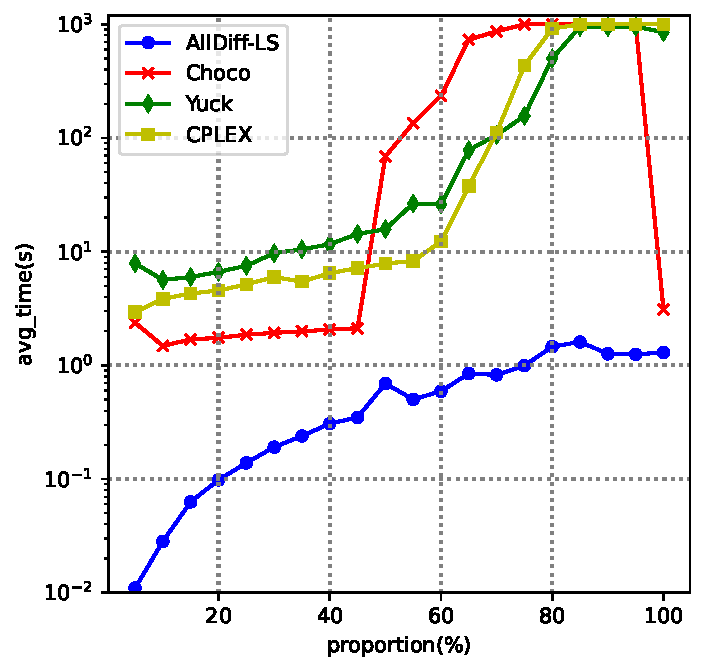
\includegraphics[width=0.55\textwidth]{Img/des.pdf}
    \bicaption {四种方法在给定基准测试上的结果。当$avg\_time$为1000s时,意味着超时。} {Results of methods on given benchmarks. when $avg\_time$ is 1000s, it means timeout.}
    \label{fig:des}
\end{figure}

本文还比较了AllDifferent约束数量对解决难度的影响。具体来说,本文选择了难度适中的实例族$\mathcal{S}$-7-0,并通过随机删除实例族的约束,按顺序得到了20个新的约束逐渐减少的实例族(累计2000个实例)(约束从原始的5\%到100\%不等)。结果如\figurename~\ref{fig:des}所示。
由于一些实例不再是数独,本文使用Yuck代替ACS和ILS。
横坐标表示约束逐渐增加的实例族,纵坐标表示每个实例族的平均时间消耗。
结果表明,随着约束数量的增加,问题的解决难度在一定比例内会急剧增加,与其他方法相比,AllDiff-LS受影响最小。

最后,本文给出额外的三个求解器:OR-Tools、LocalSolver和Kissat,出于类型原因,本文把它们的求解结果放在最后介绍。其中,Google的OR-Tools是一套开源的软件库,它包含了丰富的解决方案,可以用于求解CSP、LP、MIP等各类优化问题,是比较新的开源求解工具,并且支持多线程求解;LocalSolver是一款基于局部搜索的优化求解器,专门设计用来解决各种复杂的组合优化问题,它是一款商业求解器,同样支持多线程求解;Kissat是一款高效的SAT求解器,它的一个显著特点是它的求解策略旨在利用现代多核处理器的并行计算能力,以提高求解效率。

由于LocalSolver不支持并行运行多个实例,对于数独的每个实例族,本文仅运行其中随机的一个实例,在表中本文不给出求解比例,仅提供单个实例的求解时间作为参考。同时,由于除数独外的例子都包含变量表达式,使用SAT对其编码比较困难(需要借助加法器),所以本文仅给出数独的Kissat求解结果。这些求解器的多线程求解结果如\tablename~\ref{tab:OR-tools-1}和\tablename~\ref{tab:OR-tools-2}所示,其中数独实例仍然舍弃了容易求解的部分样例族。可以观察到,OR-Tools的求解能力最好,并且能够求解AllDiff-LS无法求解的实例$\mathcal{L}$-9,但在除此之外的其他实例上仍然不如AllDiff-LS。而将CSP编码成SAT问题再使用Kissat求解的方法,相较于OR-Tools求解器在低阶数独上效果较好,但在高阶例子上表现较差。

\begin{table}[]
    \bicaption{OR-Tools、LocalSolver和SAT求解器Kissat在数独实例上的结果。}{Results of OR-Tools, LocalSolver and SAT Solver Kissat on Sudoku.}
    \label{tab:OR-tools-1}
    \footnotesize
    \centering
    \setlength{\tabcolsep}{0.3mm}% column separation
    \renewcommand{\arraystretch}{1.2}%row space 
    \resizebox{\linewidth}{!}{
        \begin{tabular}{cccccc|cccccc|cccccc}
            \hline
            Instance & \multicolumn{2}{c}{OR-Tools} & \multicolumn{2}{c}{Kissat} & {LocalSolver} &
            Instance & \multicolumn{2}{c}{OR-Tools} & \multicolumn{2}{c}{Kissat} & {LocalSolver} &
            Instance & \multicolumn{2}{c}{OR-Tools} & \multicolumn{2}{c}{Kissat} & {LocalSolver} \\
            family  &  $R(\%)$ & $time$  &  $R(\%)$ & $time$  & $time$  &
            family  &  $R(\%)$ & $time$  &  $R(\%)$ & $time$  & $time$  &
            family  &  $R(\%)$ & $time$  &  $R(\%)$ & $time$  & $time$  \\
            \hline
            $\mathcal{S}$-4-0 & $100$ & $1.06$ & $100$ & $0.03$ & $0.79$ &
            $\mathcal{S}$-6-0 & $100$ & $101.77$ & $100$ & $3.51$ & $12.71$ &
            $\mathcal{S}$-8-0 & $100$ & $230.82$ & $100$ & $5.05$ & $-$ \\

            $\mathcal{S}$-4-10 & $100$ & $0.81$ & $100$ & $0.04$ & $0.84$ &
            $\mathcal{S}$-6-10 & $100$ & $70.36$ & $100$ & $12.90$ & $19.32$ &
            $\mathcal{S}$-8-10 & $98$ & $396.82$ & $0$ & $-$ & $-$ \\

            $\mathcal{S}$-4-20 & $100$ & $0.67$ & $100$ & $0.04$ & $0.55$ &
            $\mathcal{S}$-6-20 & $100$ & $15.78$ & $100$ & $12.38$ & $95.83$ &
            $\mathcal{S}$-8-20 & $99$ & $295.43$ & $0$ & $-$ & $-$ \\

            $\mathcal{S}$-4-30 & $100$ & $0.58$ & $100$ & $0.03$ & $0.51$ &
            $\mathcal{S}$-6-30 & $100$ & $7.45$ & $100$ & $11.45$ & $307.31$ &
            $\mathcal{S}$-8-30 & $100$ & $229.50$ & $0$ & $-$ & $-$ \\

            $\mathcal{S}$-4-40 & $100$ & $0.51$ & $100$ & $0.03$ & $0.47$ &
            $\mathcal{S}$-6-40 & $100$ & $15.71$ & $100$ & $54.29$ & $-$ &
            $\mathcal{S}$-8-40 & $10$ & $-$ & $0$ & $-$ & $-$ \\

            $\mathcal{S}$-4-50 & $100$ & $0.03$ & $100$ & $0.03$ & $0.22$ &
            $\mathcal{S}$-6-50 & $80$ & $255.22$ & $100$ & $475.99$ & $-$ &
            $\mathcal{S}$-8-50 & $0$ & $-$ & $0$ & $-$ & $-$ \\

            $\mathcal{S}$-5-0 & $100$ & $8.89$ & $100$ & $0.33$ & $3.69$ &
            $\mathcal{S}$-7-0 & $100$ & $386.07$ & $100$ & $88.60$ & $49.62$ &
            $\mathcal{S}$-9-0 & $0$ & $-$ & $0$ & $-$ & $-$ \\
            
            $\mathcal{S}$-5-10 & $100$ & $2.64$ & $100$ & $0.36$ & $4.56$ &
            $\mathcal{S}$-7-10 & $100$ & $213.12$ & $95$ & $264.54$ & $83.90$ &
            $\mathcal{S}$-9-10 & $0$ & $-$ & $0$ & $-$ & $-$ \\

            $\mathcal{S}$-5-20 & $100$ & $1.53$ & $100$ & $0.65$ & $9.36$ &
            $\mathcal{S}$-7-20 & $100$ & $216.22$ & $83$ & $307.86$ & $605.231$ &
            $\mathcal{S}$-9-20 & $0$ & $-$ & $0$ & $-$ & $-$ \\

            $\mathcal{S}$-5-30 & $100$ & $1.26$ & $100$ & $0.72$ & $35.66$ &
            $\mathcal{S}$-7-30 & $100$ & $143.73$ & $42$ & $289.48$ & $-$ &
            $\mathcal{S}$-9-30 & $0$ & $-$ & $0$ & $-$ & $-$ \\

            $\mathcal{S}$-5-40 & $100$ & $1.08$ & $100$ & $1.40$ & $65.53$ &
            $\mathcal{S}$-7-40 & $76$ & $-$ & $0$ & $-$ & $-$ &
            $\mathcal{S}$-9-40 & $0$ & $-$ & $0$ & $-$ & $-$ \\

            $\mathcal{S}$-5-50 & $100$ & $0.53$ & $100$ & $0.52$ & $5.03$ &
            $\mathcal{S}$-7-50 & $0$ & $-$ & $0$ & $-$ & $-$ &
            $\mathcal{S}$-9-50 & $0$ & $-$ & $0$ & $-$ & $-$ \\
            
            \hline
        \end{tabular}
    }
\end{table}

\begin{table}[]
    \bicaption{OR-Tools和LocalSolver在其他实例上的结果。}{Results of OR-Tools and LocalSolver on other benchmarks.}
    \label{tab:OR-tools-2}
    \footnotesize
    \centering
    \setlength{\tabcolsep}{0.4mm}% column separation
    \renewcommand{\arraystretch}{1.2}%row space 
    \resizebox{\linewidth}{!}{
        \begin{tabular}{ccc|ccc|ccc|ccc}
            \hline
            Instance & {OR-Tools} & {LocalSolver} & 
            Instance & {OR-Tools} & {LocalSolver} & 
            Instance & {OR-Tools} & {LocalSolver} &
            Instance & {OR-Tools} & {LocalSolver} \\
            family  &  $time$  &  $time$  &
            family  &  $time$  &  $time$  &
            family  &  $time$  &  $time$  &
            family  &  $time$  &  $time$  \\
            
            \hline

            $\mathcal{Q}$-500 & $105.29$ & $212.35$ &
            $\mathcal{Q}$-2000 & $-$ & $-$ &
            $\mathcal{Q}$-3500 & $-$ & $-$ &
            $\mathcal{Q}$-5000 & $-$ & $-$ \\
            
            $\mathcal{Q}$-1000 & $559.75$ & $-$ &
            $\mathcal{Q}$-2500 & $-$ & $-$ &
            $\mathcal{Q}$-4000 & $-$ & $-$ &
            $\mathcal{Q}$-5500 & $-$ & $-$ \\

            $\mathcal{Q}$-1500 & $-$ & $-$ &
            $\mathcal{Q}$-3000 & $-$ & $-$ &
            $\mathcal{Q}$-4500 & $-$ & $-$ &
            $\mathcal{Q}$-6000 & $-$ & $-$ \\
            
            \hline

            % $\mathcal{A}$-10 & $0.35$ & $0.14$ &
            $\mathcal{A}$-12 & $0.94$ & $0.14$ &
            $\mathcal{A}$-16 & $0.60$ & $0.20$ &
            $\mathcal{A}$-20 & $0.73$ & $0.22$ &
            $\mathcal{A}$-24 & $0.93$ & $0.25$ \\
            
            $\mathcal{A}$-14 & $0.56$ & $0.14$ &
            $\mathcal{A}$-18 & $0.66$ & $0.22$ &
            $\mathcal{A}$-22 & $0.88$ & $0.23$ &
            $\mathcal{A}$-26 & $1.05$ & $0.24$ \\

            \hline

            $\mathcal{L}$-3 & $0.89$ & $0.15$ &
            $\mathcal{L}$-5 & $0.51$ & $0.20$ &
            $\mathcal{L}$-8 & $13.41$ & $-$ \\

            $\mathcal{L}$-4 & $0.37$ & $0.16$ &
            $\mathcal{L}$-7 & $6.37$ & $17.55$ &
            $\mathcal{L}$-9 & $63.69$ & $-$ \\
   
            \hline
        \end{tabular}
    }
\end{table}

\section{AllDiff-LS涉及的策略的有效性}

本文首先研究两个简化规则的有效性。由于N-queens和2-MOLS的ACG无法被简化,本文在数独实例上进行了实验,其中推理规则的效果是非琐碎的(去除了填充比例小于40\%的实例)。结果如\tablename~\ref{tab:rule}所示,其中$avg$表示每个实例族变量数量的平均简化比例。可以看出,使用两个简化规则比只使用rule1或rule2更好,并且在填充率高的情况下,大部分变量都可以被简化。

\begin{table}[h]
    \bicaption{在给定数独实例上使用不同化简规则对应的变量简化比率。}{The variable simplification ratio of different simplification rules on given Sudoku.}
    \label{tab:rule}
    \footnotesize
    \centering
    \setlength{\tabcolsep}{0.4mm}% column separation
    \renewcommand{\arraystretch}{1.0}%row space 
    \resizebox{\linewidth}{!}{
        \begin{tabular}{cccc|cccc|cccc}
            \hline
            Instance & Rule1+2 & Rule1 & Rule2 &
            Instance & Rule1+2 & Rule1 & Rule2 &
            Instance & Rule1+2 & Rule1 & Rule2 \\
            family & $avg(\%)$ & $avg(\%)$ & $avg(\%)$ &
            family & $avg(\%)$ & $avg(\%)$ & $avg(\%)$ &
            family & $avg(\%)$ & $avg(\%)$ & $avg(\%)$ \\
            \hline

            $\mathcal{S}$-4-40 & \textbf{9.44} & 8.22 & 1.18 &
            $\mathcal{S}$-6-40 & \textbf{0.43} & \textbf{0.43} & 0.01 &
            $\mathcal{S}$-8-40 & \textbf{0.02} & \textbf{0.02} & 0.00 \\
            
            $\mathcal{S}$-4-50 & \textbf{79.34} & 70.41 & 27.20 & 
            $\mathcal{S}$-6-50 & \textbf{4.28} & 3.97 & 0.21 & 
            $\mathcal{S}$-8-50 & \textbf{0.48} & 0.47 & 0.01 \\
            
            $\mathcal{S}$-4-60 & \textbf{94.91} & 94.90 & 93.95 & 
            $\mathcal{S}$-6-60 & \textbf{96.54} & \textbf{96.54} & 10.63 & 
            $\mathcal{S}$-8-60 & \textbf{7.10} & 6.42 & 0.41 \\
            
            $\mathcal{S}$-4-70 & \textbf{95.29} & \textbf{95.29} & 95.28 & 
            $\mathcal{S}$-6-70 & \textbf{98.93} & \textbf{98.93} & \textbf{98.93} & 
            $\mathcal{S}$-8-70 & \textbf{99.12} & \textbf{99.12} & 99.09 \\
            
            $\mathcal{S}$-4-80 & \textbf{91.06} & \textbf{91.06} & \textbf{91.06} & 
            $\mathcal{S}$-6-80 & \textbf{98.10} & \textbf{98.10} & 98.09 & 
            $\mathcal{S}$-8-80 & \textbf{99.40} & \textbf{99.40} & \textbf{99.40} \\
            
            $\mathcal{S}$-4-90 & \textbf{82.96} & \textbf{82.96} & \textbf{82.96} & 
            $\mathcal{S}$-6-90 & \textbf{93.78} & \textbf{93.78} & \textbf{93.78} & 
            $\mathcal{S}$-8-90 & \textbf{97.22} & \textbf{97.22} & \textbf{97.22} \\
            
            $\mathcal{S}$-5-40 & \textbf{1.53} & 1.42 & 0.09 & 
            $\mathcal{S}$-7-40 & \textbf{0.09} & \textbf{0.09} & 0.00 &
            $\mathcal{S}$-9-40 & \textbf{0.01} & \textbf{0.01} & 0.00 \\
            
            $\mathcal{S}$-5-50 & \textbf{20.92} & 14.69 & 2.25 & 
            $\mathcal{S}$-7-50 & \textbf{1.35} & 1.31 & 0.04 &
            $\mathcal{S}$-9-50 & \textbf{0.16} & \textbf{0.16} & 0.00 \\
            
            $\mathcal{S}$-5-60 & \textbf{95.98} & 95.92 & 83.16 & 
            $\mathcal{S}$-7-60 & \textbf{43.80} & 18.48 & 1.63 &
            $\mathcal{S}$-9-60 & \textbf{3.05} & 2.92 & 0.10 \\
            
            $\mathcal{S}$-5-70 & \textbf{97.65} & \textbf{97.65} & 97.64 & 
            $\mathcal{S}$-7-70 & \textbf{99.11} & \textbf{99.11} & 99.10 &
            $\mathcal{S}$-9-70 & \textbf{99.31} & 99.30 & 15.45 \\
            
            $\mathcal{S}$-5-80 & \textbf{95.54} & \textbf{95.54} & \textbf{95.54} & 
            $\mathcal{S}$-7-80 & \textbf{98.90} & \textbf{98.90} & 98.90 &
            $\mathcal{S}$-9-80 & \textbf{99.56} & \textbf{99.56} & \textbf{99.56} \\
            
            $\mathcal{S}$-5-90 & \textbf{89.42} & \textbf{89.42} & \textbf{89.42} & 
            $\mathcal{S}$-7-90 & \textbf{95.95} & \textbf{95.95} & \textbf{95.95} &
            $\mathcal{S}$-9-90 & \textbf{98.28} & \textbf{98.28} & \textbf{98.28} \\
            
            \hline
        \end{tabular}
    }
\end{table}

此外,需要对文章中提到的主要策略进行消融实验,本文将实验分为了两大组,一组用来研究移动选择方法和重启策略的影响,而另一组用于展示了禁忌策略1、禁忌策略3和打破平局技术对算法解决效率的影响。

第一组实验结果如\figurename~\ref{fig:Compare}所示,每个点代表一个随机种子实验。为了使结果更清晰,对于数独实验,本文选择了五个困难的实例族($\mathcal{S}$-6-50、$\mathcal{S}$-7-50、$\mathcal{S}$-8-50、$\mathcal{S}$-8-60和$\mathcal{S}$-9-50),一个点代表十个随机种子实验的结果,其中运行时间是它们运行时间的平均值。其中,AllDiff-LS-DM用直接移动选择方法替换了本文的移动选择策略;在AllDiff-LS-FL中,使用固定数量的内循环迭代替代动态迭代,并从算法~\ref{alg:SelectSolution}中移除权重策略。可见,在数独问题上,AllDiff-LS-DM的性能在几乎所有实例中都比AllDiff-LS弱,从运行时间的比较中可以观察到移动选择策略的有效性。此外,AllDiff-LS-FL在耗时的数独实例中表现出劣势。在其他三种类型的问题上,AllDiff-LS对AllDiff-LS-DM的优势仍然存在,但由于一些实例的规模较小,AllDiff-LS对AllDiff-LS-FL的效率提升不明显。

在\figurename~\ref{fig:ablation}中,本文展示了其他策略对数独实例的提升效果。具体的,相较于原AllDiff-LS算法,在AllDiff-LS-TA中本文将策略1替换为了传统的tabu策略,在AllDiff-LS-SW中本文删除了策略3,而在AllDiff-LS-BT中本文删除了打破平局的策略。AllDiff-LS-TA算法在一些较难的例子上会出现循环,因此求解会超时。

\begin{figure}[t]
    \centering
    {%
        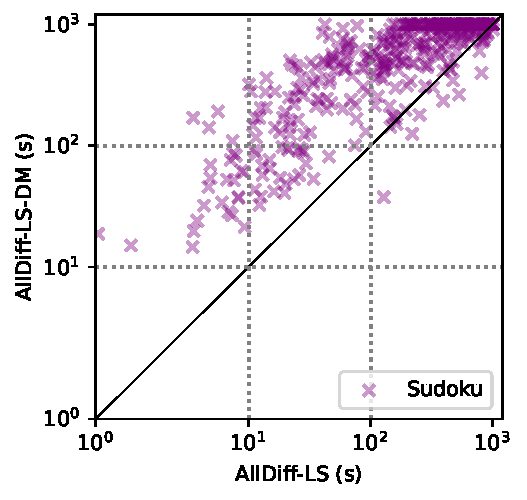
\includegraphics[width=.50\linewidth]{Img/Sudoku_DM.pdf}%
        % \label{compare_1}%
    }\hfill	
    {%
        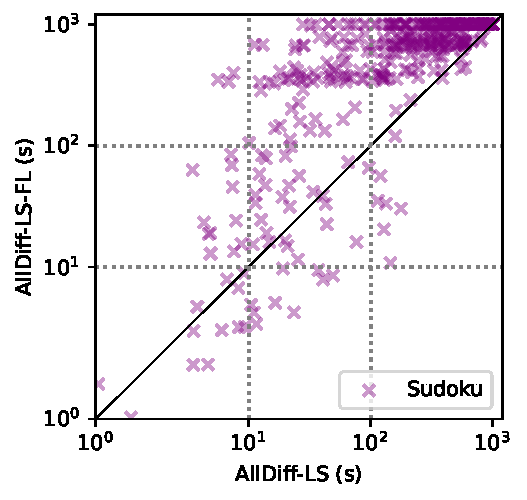
\includegraphics[width=.50\linewidth]{Img/Sudoku_FL.pdf}%
        % \label{compare_2}%
    }\\
    {%
        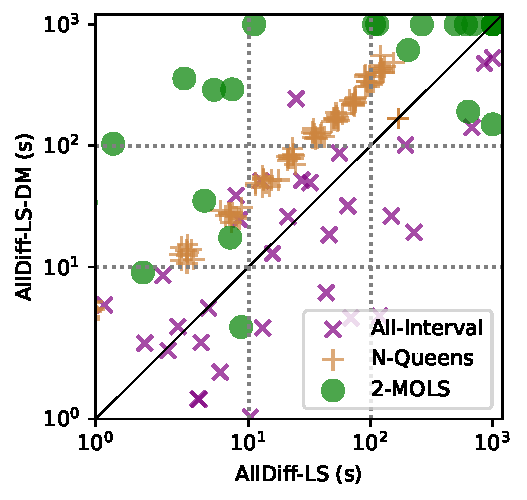
\includegraphics[width=.50\linewidth]{Img/Others_DM.pdf}%
        % \label{compare_3}%
    }\hfill	
    {%
        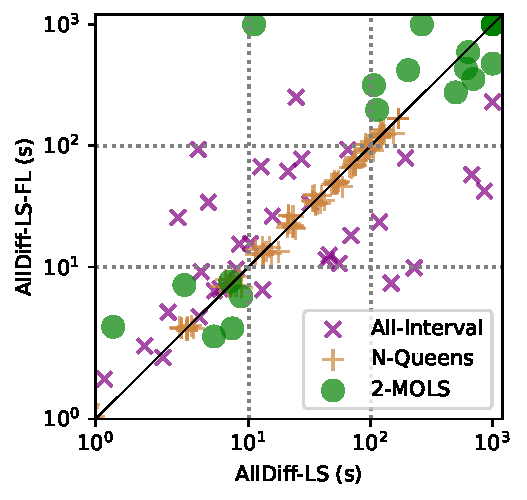
\includegraphics[width=.50\linewidth]{Img/Others_FL.pdf}%
        % \label{compare_4}%
    }
\bicaption {在四类实例上AllDiff-LS(横坐标)和其他两个版本(纵坐标)的平均运行时间比较。} {Comparison of the average running time of AllDiff-LS (abscissa) and the other two versions (ordinate) on four kinds of benchmarks.}
\label{fig:Compare}
\end{figure}

\begin{figure}[]
    \centering
    {%
        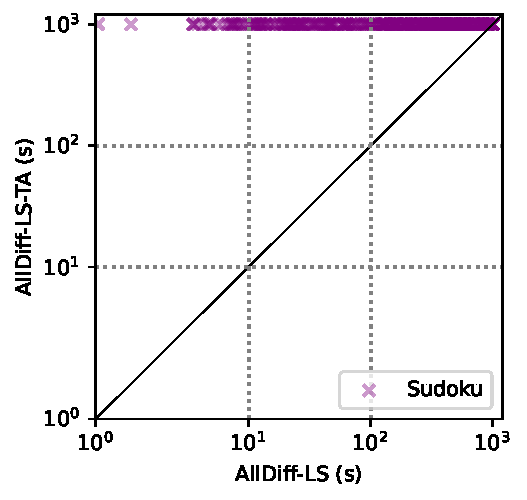
\includegraphics[width=.33\linewidth]{Img/AllDiff-LS_VS_AllDiff-LS-TA(log).pdf}%
        % \label{compare_1}%
    }\hfill	
    {%
        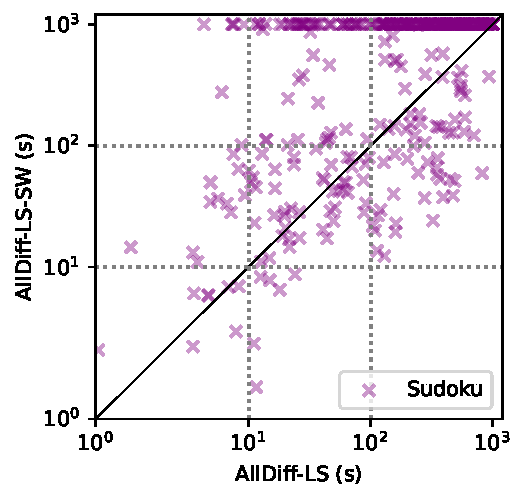
\includegraphics[width=.33\linewidth]{Img/AllDiff-LS_VS_AllDiff-LS-SW(log).pdf}%
        % \label{compare_2}%
    }\hfill	
    {%
        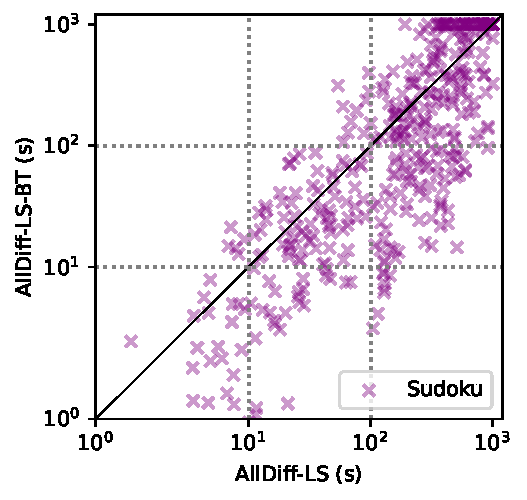
\includegraphics[width=.33\linewidth]{Img/AllDiff-LS_VS_AllDiff-LS-BT(log).pdf}%
        % \label{compare_3}%
    }\\
\bicaption {在数独上AllDiff-LS(横坐标)与其他三个版本(纵坐标)的平均运行时间比较。} {Comparison of the average running time of AllDiff-LS (abscissa) and the other three versions (ordinate) on Sudoku benchmarks.}
\label{fig:ablation}
\end{figure}

\clearpage

\section{本章小结}

本章节通过设计实验,对基于AllDiff-LS算法实现的求解工具进行了深入的性能评估和策略分析。
在第一节中,本文详细介绍了实验的安排,包括所使用的数据集和比较的方法。
在第二节中,本文展示了算法在多个实验基准上与其他方法的性能比较结果,证明了其优越的性能。
在第三节中,本文通过消融实验,对实验中提到的各种策略的有效性进行了验证。
实验结果表明,基于AllDiff-LS算法实现的求解工具在处理各类问题时都展现出了强大的性能,证明了本文选择和实施的策略的有效性。